% Provenance (never printed): see sources/outline_sources.md (Year 3: the
% Rayleigh number; thermal boundary layers; slab pull and ridge push; plumes;
% post-glacial rebound and mantle viscosity). Brief: sources/book5/BRIEFS.md,
% ch. 6. Curves from figdata/bachelor-3/convection_scaling.py (PREM read only),
% gia_relaxation.py and ridge_push.py (on plate_cooling.py). Exercise and
% problem values in the Book 5 scratch calculator calc/ch06.py.
\chapter{Konveksi Mantel dan Gaya Penggerak Lempeng}\label{ch:b3:mantle-convection}

Pesisir utara Swedia naik dari laut sekitar satu sentimeter per
tahun, sepuluh ribu tahun setelah lembaran es yang menutupinya mencair; pantai
Teluk Hudson naik sama cepatnya. Tidak ada yang mendorong mereka ke atas selain mantel,
yang perlahan mengalir kembali di bawah tempat yang semula ditekan es. Laju
ketika tanah memantul kembali menakar \omterm{def:b3:mantle-convection:gia}{viskositas mantel}, dan viskositas
yang sama juga menentukan seberapa cepat mantel berkonveksi dan lempeng bergerak. Bab ini
menanyakan mengapa mantel padat berkonveksi sama sekali, seberapa cepat ia harus mengalir
untuk membawa panas Bumi, gaya apa yang menggerakkan lempeng, dan apa yang
diungkap pantulan tanah tentang \omterm{def:b3:mantle-convection:gia}{viskositas mantel}.
% ledger: vestol19:umea, zhao12:fenno, sella07:gia

\begin{recall}
Viskositas, aliran merayap fluida kental (persamaan Stokes
$\nabla p = \eta\nabla^2\mathbf u$, $\nabla\cdot\mathbf u = 0$), hukum Stokes
untuk bola, bilangan Reynolds, dan daya apung terdapat dalam
volume universitas buku fisika. Konveksi mantel dan pantulan isostatik dibahas
dalam volume sekolah menengah atas (kelas 12); dorongan punggung dan tarikan lempengan di bagian kelas 11.
Lapisan batas termal, litosfer termal, dan adiabat mantel terdapat
dalam volume Tahun 1, pada bab tentang anggaran panas Bumi; titik panas,
plume mantel dan provinsi beku besar dalam bab tentang titik panas. \omterm{def:b3:lithosphere-thermal-models:half-space}{Model
pendinginan setengah-ruang} terdapat pada \cref{ch:b3:lithosphere-thermal-models},
\omterm{def:b3:gravity-geodesy:flexure}{lenturan litosfer} ada pada \cref{ch:b3:gravity-geodesy}, serta
\omterm{def:b3:seismology-imaging:tomography}{tomografi seismik} pada \cref{ch:b3:seismology-imaging}.
\end{recall}

\section{Mengapa mantel berkonveksi}

Mantel bersifat padat: ia meneruskan gelombang S. Namun, dalam jutaan tahun, ia
merayap seperti fluida dengan viskositas sangat besar, dan lapisan fluida yang dipanaskan dari
bawah dan didinginkan dari atas dapat tetap diam, dengan panas melintasinya secara
konduksi, atau berpusar. Gumpalan fluida panas berukuran $d$, yang lebih ringan daripada
lingkungannya sebesar $\rho\alpha\,\Delta T$, naik dengan laju berorde
$\rho g\alpha\,\Delta T d^2/\eta$; ia kehilangan panas melalui difusi dalam waktu
berorde $d^2/\kappa$. Jika ia dapat naik melintasi lapisan sebelum mendingin, lapisan itu
berpusar.

\begin{definition}[Bilangan Rayleigh]\label{def:b3:mantle-convection:rayleigh}
Untuk lapisan fluida dengan ketebalan $d$, massa jenis $\rho$, koefisien muai termal
$\alpha$, difusivitas termal $\kappa$, dan viskositas $\eta$, di bawah
gravitasi $g$, dengan selisih suhu $\Delta T$ antara dasarnya dan
puncaknya, \emph{bilangan Rayleigh}\index{bilangan Rayleigh} adalah
\[
  \mathrm{Ra} = \frac{\rho g\alpha\,\Delta T d^3}{\kappa\eta},
\]
rasio waktu difusi $d^2/\kappa$ terhadap waktu naik karena daya apung
$\eta/(\rho g\alpha\,\Delta Td)$.
\end{definition}

\begin{definition}[Bilangan Rayleigh kritis]\label{def:b3:mantle-convection:critical}
Yang disebut \emph{bilangan Rayleigh kritis}\index{bilangan Rayleigh kritis}
$\mathrm{Ra}_c$ suatu lapisan adalah nilai \omterm{def:b3:mantle-convection:rayleigh}{bilangan Rayleigh} yang bila terlampaui,
gangguan kecil pada keadaan diam tumbuh menjadi konveksi, dan di bawahnya
gangguan itu mereda.
\end{definition}

\begin{proposition}[Permulaan konveksi]\label{prop:b3:mantle-convection:onset}
Untuk lapisan yang puncak dan dasarnya bebas dari tegangan geser dan dijaga
pada suhu tetap, gangguan dengan bilangan gelombang horizontal $k$ (dalam satuan $1/d$)
tumbuh bila $\mathrm{Ra} > (\pi^2 + k^2)^3/k^2$. Nilai minimum ruas kanan
itu, pada $k = \pi/\sqrt2$, memberikan
\[
  \mathrm{Ra}_c = \frac{27\pi^4}{4} \approx 657.5,
\]
dan sel pertama yang muncul selebar $2\sqrt2\,d$. Di antara batas kaku,
$\mathrm{Ra}_c \approx 1708$.
\end{proposition}

\admitted
Analisis stabilitas linear yang mendasarinya, yakni perturbasi persamaan panas
dan Stokes terhadap keadaan konduktif, terdapat dalam pembahasan
konveksi di buku fisika; latihan 11 memeriksa nilai minimumnya.

Gambar di bawah memperlihatkan lapisan yang berkonveksi. Nilai untuk mantel, beserta
kedalaman batas inti--mantel, $d = \qty{2891}{km}$, massa jenis rata-rata
mantel, \qty{4476}{kg.m^{-3}}, dan $g$ antara 9.8 dan
\qty{10.7}{m.s^{-2}}, semuanya dari model Bumi seismik PREM; $\alpha =
\qty{3.1e-5}{K^{-1}}$ dan $\Delta T = \qty{1450}{K}$ dari model lempeng pada
\cref{ch:b3:lithosphere-thermal-models}; $\kappa = \qty{e-6}{m^2.s^{-1}}$;
dan $\eta$ antara \num{e21} dan \qty{e22}{Pa.s} (\cref{sec:b3:mantle-convection:gia}),
memberikan $\mathrm{Ra}$ antara \num{4.9e6} dan \num{4.9e7}, sekitar tujuh ribu hingga
tujuh puluh ribu kali nilai kritis. Mantel tak mungkin tidak berkonveksi.
% ledger: data:prem, honda04:gdh1, delaney86:properties, mitrovica96:haskell, milne04:bifrost

\begin{omfigure}
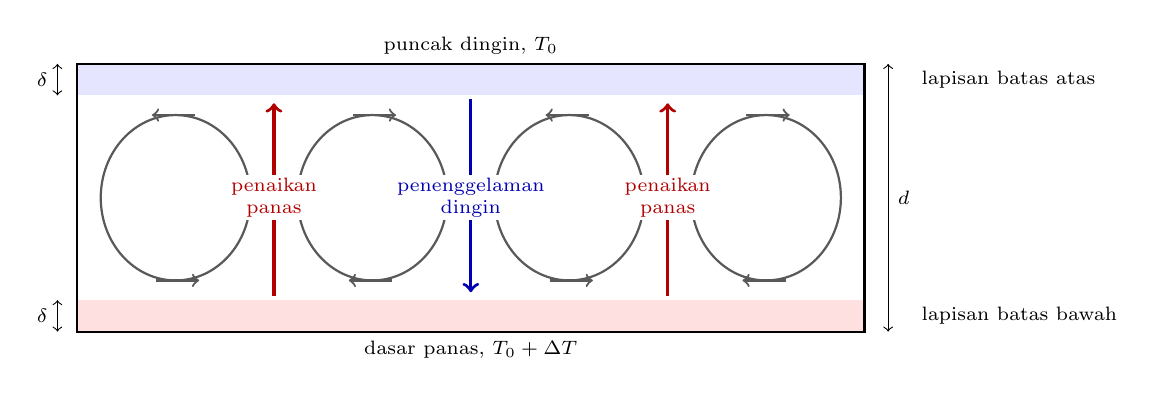
\begin{tikzpicture}[font=\scriptsize, x=1cm, y=1cm]
\fill[blue!10] (0,3.4) rectangle (10,3.0);
\fill[red!12] (0,0) rectangle (10,0.4);
\draw[thick] (0,0) rectangle (10,3.4);
\node[above] at (5,3.4) {puncak dingin, $T_0$};
\node[below] at (5,0) {dasar panas, $T_0 + \Delta T$};
\foreach \c/\s in {1.25/1, 3.75/-1, 6.25/1, 8.75/-1} {
  \draw[gray!70!black, thick] (\c,1.7) ellipse[x radius=0.95, y radius=1.05];
  \draw[->, gray!70!black, thick] ({\c+0.25*\s},2.75) -- ({\c-0.3*\s},2.75);
  \draw[->, gray!70!black, thick] ({\c-0.25*\s},0.65) -- ({\c+0.3*\s},0.65);
}
\draw[->, red!70!black, very thick] (2.5,0.45) -- (2.5,2.9);
\draw[->, red!70!black, very thick] (7.5,0.45) -- (7.5,2.9);
\draw[->, blue!70!black, very thick] (5,2.95) -- (5,0.5);
\node[red!70!black, fill=white, inner sep=1pt, align=center] at (2.5,1.7) {penaikan\\panas};
\node[red!70!black, fill=white, inner sep=1pt, align=center] at (7.5,1.7) {penaikan\\panas};
\node[blue!70!black, fill=white, inner sep=1pt, align=center] at (5,1.7) {penenggelaman\\dingin};
\draw[<->] (10.3,0) -- (10.3,3.4) node[midway, right] {$d$};
\draw[<->] (-0.25,3.0) -- (-0.25,3.4) node[midway, left] {$\delta$};
\draw[<->] (-0.25,0) -- (-0.25,0.4) node[midway, left] {$\delta$};
\node[anchor=west] at (10.6,3.2) {lapisan batas atas};
\node[anchor=west] at (10.6,0.2) {lapisan batas bawah};
\end{tikzpicture}

\par\smallskip{\small Konveksi dalam lapisan yang dipanaskan dari bawah dan didinginkan dari
atas. Panas melintasi lapisan batas yang tipis, setebal $\delta$, secara
konduksi; di antaranya, bagian dalam yang tercampur baik membawa panas dengan aliran. Lembaran dingin
lepas dari lapisan atas dan tenggelam; yang panas naik dari
bawah.}\label{fig:b3:mantle-convection:cell}
\end{omfigure}

Mantel juga dipanaskan dari dalam, oleh peluruhan unsur-unsur radioaktif,
dan dari bawah, oleh inti. Lapisan yang hanya dipanaskan dari dalam tidak memiliki
lapisan batas panas di dasarnya: alirannya digerakkan oleh lembaran dingin yang tenggelam dari
atas, sedangkan aliran naik berupa arus balik yang lebar dan pasif. Lempengan termasuk lembaran semacam itu, dan
plume membutuhkan panas dari inti.

\section{Lapisan batas dan kekuatan konveksi}

\begin{definition}[Bilangan Nusselt]\label{def:b3:mantle-convection:nusselt}
Yang disebut \emph{bilangan Nusselt}\index{bilangan Nusselt} suatu lapisan yang berkonveksi adalah
aliran panas yang melewatinya dibagi aliran panas yang dibawa konduksi saja
pada lapisan yang sama, $\mathrm{Nu} = q\,d/(k\,\Delta T)$.
\end{definition}

\begin{theorem}[Penskalaan lapisan batas konveksi]\label{thm:b3:mantle-convection:scaling}
Dalam lapisan yang berkonveksi pada $\mathrm{Ra} \gg \mathrm{Ra}_c$, jika setiap lapisan batas termal
tumbuh hingga \omterm{def:b3:mantle-convection:rayleigh}{bilangan Rayleigh-nya} sendiri, yang dihitung dari tebalnya
$\delta$ dan beda suhu $\Delta T/2$ melintasinya, mencapai
$\mathrm{Ra}_c$, maka
\[
  \delta = d\Bigl(\frac{2\mathrm{Ra}_c}{\mathrm{Ra}}\Bigr)^{1/3},\qquad
  \mathrm{Nu} = \frac12\Bigl(\frac{\mathrm{Ra}}{2\mathrm{Ra}_c}\Bigr)^{1/3},
  \qquad
  u = \frac\kappa d\Bigl(\frac{\mathrm{Ra}}{2\mathrm{Ra}_c}\Bigr)^{2/3},
\]
Di sini $u$ adalah skala kecepatan aliran, yang didefinisikan dengan mensyaratkan bahwa
lapisan tumbuh hingga $\delta$ selagi fluida melintasi sel.
Inilah yang disebut \emph{penskalaan lapisan batas konveksi}\index{penskalaan lapisan batas konveksi}.
\end{theorem}

\begin{proof}
Bagian dalam tercampur baik, pada suhu rata-rata, sehingga setiap lapisan batas
membawa setengah dari $\Delta T$. \omterm{def:b3:mantle-convection:rayleigh}{Bilangan Rayleigh-nya} adalah $\rho g\alpha(\Delta T/2)
\delta^3/(\kappa\eta) = \mathrm{Ra}\,(\delta/d)^3/2$; dengan menyamakannya dengan
$\mathrm{Ra}_c$ memberikan $\delta$. Aliran panas dihantarkan melintasi lapisan,
$q = k(\Delta T/2)/\delta$, sehingga $\mathrm{Nu} = qd/(k\Delta T) = d/(2\delta)$.
Lapisan batas tumbuh secara difusi hingga tebal $\delta$ dalam waktu
$\delta^2/\kappa$; fluida di bagian atas melintasi sel yang lebarnya berorde
$d$, dalam waktu $d/u$. Dengan menyamakan kedua waktu itu, $u = \kappa d/\delta^2 =
(\kappa/d)(d/\delta)^2$.
\end{proof}

Aliran panas hanya tumbuh sebagai akar pangkat tiga dari $\mathrm{Ra}$: viskositas seratus kali
lebih rendah, panas kurang dari lima kali lebih banyak. Untuk mantel dengan
$\mathrm{Ra} = \num{4.9e7}$, penskalaan memberikan $\delta \approx \qty{87}{km}$,
$\mathrm{Nu} \approx 17$, aliran panas sebesar $\mathrm{Nu}\,k\Delta T/d \approx
\qty{26}{mW.m^{-2}}$ dengan $k = \qty{3.1}{W.m^{-1}.K^{-1}}$, dan $u \approx
\qty{1.2}{cm/yr}$ (gambar di bawah). Tebal lapisan batas sama dengan
lempeng samudra pada \cref{ch:b3:lithosphere-thermal-models}, \qty{95}{km}; kecepatan
akar rata-rata kuadrat lempeng masa kini berkisar dari \qty{1.1}{cm/yr} (Amerika
Selatan) hingga \qty{7.5}{cm/yr} (Cocos), \qty{4.4}{cm/yr} untuk seluruh
litosfer. Aliran panas rata-rata Bumi, \qty{92}{mW.m^{-2}}, adalah tiga sampai empat
kali hasil penskalaan: panas yang dihasilkan di dalam mantel, yang tidak
diperhitungkan lapisan yang dipanaskan dari bawah, serta konstanta berorde satu yang
diabaikan penskalaan; keduanya ikut berperan. Untuk hukum dengan satu masukan, orde besarannya
tepat: lempeng merupakan lapisan batas atas mantel dengan $\mathrm{Ra}
\sim 10^7$.
% ledger: nnr56:rms, b2dd10:continents, honda04:gdh1

\begin{omfigure}
\begin{tikzpicture}
\begin{groupplot}[group style={group size=1 by 2, vertical sep=2.5cm},
  omrecord, width=0.86\linewidth, height=0.40\linewidth, xmode=log, ymode=log,
  xmin=100, xmax=1e10, xlabel={bilangan Rayleigh $\mathrm{Ra}$}]
\nextgroupplot[ylabel={bilangan Nusselt}, ymin=0.3, ymax=300,
  title={(a) aliran panas, dalam satuan aliran konduktif}, title style={font=\small}]
% computed in figdata/bachelor-3/convection_scaling.py; ledger: data:prem, honda04:gdh1
\addplot[omDef, thick] table[x=ra, y=nu] {figdata/out/bachelor-3-convection_scaling-conduction.dat};
\addplot[red!70!black, thick] table[x=ra, y=nu] {figdata/out/bachelor-3-convection_scaling-scaling.dat};
\addplot[gray, densely dashed, unbounded coords=jump] table[x=ra, y=y] {figdata/out/bachelor-3-convection_scaling-band.dat};
\draw[gray, densely dotted] (axis cs:657.5,0.3) -- (axis cs:657.5,1);
\node[font=\scriptsize, anchor=west] at (axis cs:700,0.45) {$\mathrm{Ra}_c$};
\node[font=\scriptsize, anchor=south west, omDef] at (axis cs:115,1.08) {konduksi};
\node[font=\scriptsize, anchor=north west, red!70!black] at (axis cs:3e4,0.95) {$\tfrac12(\mathrm{Ra}/2\mathrm{Ra}_c)^{1/3}$};
\node[font=\scriptsize, fill=white, inner sep=1pt] at (axis cs:1.55e7,120) {mantel};
\nextgroupplot[ylabel={kecepatan (\unit{cm/yr})}, ymin=1e-3, ymax=100,
  title={(b) skala kecepatan untuk $d = \qty{2891}{km}$}, title style={font=\small}]
\addplot[red!70!black, thick] table[x=ra, y=u] {figdata/out/bachelor-3-convection_scaling-scaling.dat};
\addplot[gray, densely dashed, unbounded coords=jump] table[x=ra, y=y] {figdata/out/bachelor-3-convection_scaling-band.dat};
\addplot[blue!70, thick, dash dot, unbounded coords=jump] table[x=ra, y=u] {figdata/out/bachelor-3-convection_scaling-plates.dat};
\node[font=\scriptsize, anchor=south west, blue!60!black] at (axis cs:150,7.6) {lempeng tercepat};
\node[font=\scriptsize, anchor=north west, blue!60!black] at (axis cs:150,1.0) {lempeng paling lambat};
\node[font=\scriptsize, fill=white, inner sep=1pt] at (axis cs:1.55e7,0.004) {mantel};
\end{groupplot}
\end{tikzpicture}

\par\smallskip{\small Penskalaan konveksi. (a) Di bawah $\mathrm{Ra}_c$ lapisan
menghantarkan panas secara konduksi ($\mathrm{Nu} = 1$); jauh di atasnya, hukum lapisan batas, yang digambar
dari $\mathrm{Ra} = 16\,\mathrm{Ra}_c \approx \num{1.1e4}$, tempat hukum itu memberikan $\mathrm{Nu} = 1$ (di antaranya,
konveksi berangsur mulai). (b) Skala kecepatan
untuk kedalaman mantel dan $\kappa = \qty{e-6}{m^2.s^{-1}}$, dengan
rentang kecepatan lempeng masa kini (garis titik-strip). Garis putus-putus membatasi
\omterm{def:b3:mantle-convection:rayleigh}{bilangan Rayleigh} mantel untuk viskositas \num{e22} dan \qty{e21}{Pa.s}.}\label{fig:b3:mantle-convection:scaling}
\end{omfigure}

\section{Gaya-gaya pada lempeng}

Lempeng bergerak dengan kecepatan tetap: gaya-gaya padanya berada dalam keseimbangan. Tiga gaya mendorong atau
menahannya dari tepi dan dasarnya (gambar di bawah). Gaya yang
diberikan lempengan yang tenggelam pada lempengnya, yakni tarikan lempengan, berasal dari
kelebihan massa jenis lempengan dingin di dalam mantel yang lebih panas. Dorongan punggung,
yakni dorongan punggungan yang tinggi dan panas terhadap lempeng yang lebih dingin di sebelahnya, diturunkan dari \omterm{def:b3:lithosphere-thermal-models:half-space}{model pendinginan setengah-ruang} pada
\cref{ch:b3:lithosphere-thermal-models}.

\begin{omfigure}
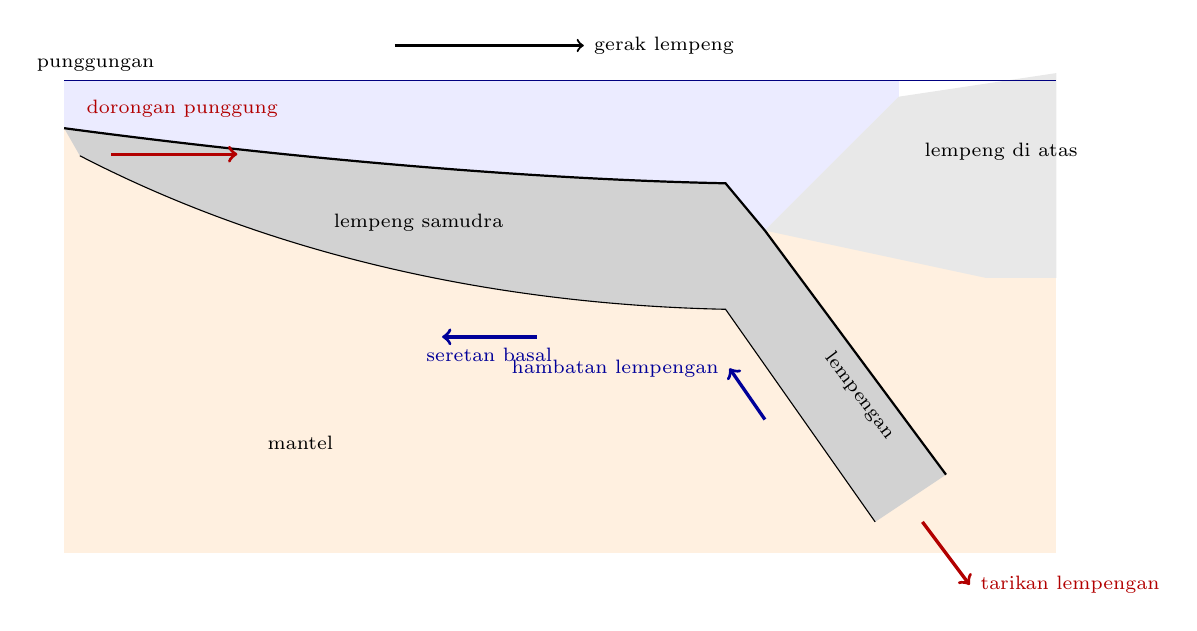
\begin{tikzpicture}[font=\scriptsize, x=1cm, y=1cm]
\fill[orange!12] (0,-0.6) rectangle (12.6,-6.0);
\fill[blue!8] (0,0) -- (0,-0.6) .. controls (3,-1.0) and (6,-1.25) .. (8.4,-1.3) -- (8.9,-1.9) -- (10.6,-0.2) -- (10.6,0) -- cycle;
\fill[gray!35] (0,-0.6) .. controls (3,-1.0) and (6,-1.25) .. (8.4,-1.3) -- (8.9,-1.9) -- (11.2,-5.0) -- (10.3,-5.6) -- (8.4,-2.9) .. controls (6,-2.85) and (3,-2.4) .. (0.2,-0.95) -- cycle;
\fill[gray!18] (10.6,-0.2) -- (12.6,0.1) -- (12.6,-2.5) -- (11.7,-2.5) -- (8.9,-1.9) -- cycle;
\draw[thick] (0,-0.6) .. controls (3,-1.0) and (6,-1.25) .. (8.4,-1.3) -- (8.9,-1.9) -- (11.2,-5.0);
\draw (0.2,-0.95) .. controls (3,-2.4) and (6,-2.85) .. (8.4,-2.9) -- (10.3,-5.6);
\draw[blue!50!black] (0,0) -- (12.6,0);
\node at (0.4,0.2) {punggungan};
\node at (4.5,-1.8) {lempeng samudra};
\node at (11.9,-0.9) {lempeng di atas};
\node[rotate=-53] at (10.1,-4.0) {lempengan};
\node at (3,-4.6) {mantel};
\draw[->, very thick, red!70!black] (0.6,-0.93) -- (2.2,-0.93);
\node[red!70!black] at (1.5,-0.35) {dorongan punggung};
\draw[->, very thick, red!70!black] (10.9,-5.6) -- (11.5,-6.4) node[right] {tarikan lempengan};
\draw[->, very thick, blue!60!black] (6.0,-3.25) -- (4.8,-3.25) node[below, pos=0.5] {seretan basal};
\draw[->, very thick, blue!60!black] (8.9,-4.3) -- (8.45,-3.65) node[left] {hambatan lempengan};
\draw[->, thick] (4.2,0.45) -- (6.6,0.45) node[right] {gerak lempeng};
\end{tikzpicture}

\par\smallskip{\small Gaya-gaya pada lempeng samudra: dorongan punggung dan tarikan lempengan
mendorong lempeng (merah); seretan di dasarnya, tempat lempeng bergerak lebih cepat daripada mantel
di bawahnya, dan hambatan kental mantel terhadap lempengan yang tenggelam
menahannya (biru).}\label{fig:b3:mantle-convection:forces}
\end{omfigure}

\begin{proposition}[Gaya dorongan punggung]\label{prop:b3:mantle-convection:ridge-push}
Pada \omterm{def:b3:lithosphere-thermal-models:half-space}{model pendinginan setengah-ruang}, dengan suhu mantel $T_m$, suhu permukaan
$T_0$ dan kompensasi isostatik, gaya horizontal per satuan
panjang punggungan yang dikerjakan kolom di punggungan pada lempeng berumur $t$,
yakni \emph{gaya dorongan punggung}\index{gaya dorongan punggung}, adalah
\[
  F_{rp} = g\rho_m\alpha(T_m - T_0)\kappa t\Bigl[1 + \frac{2\rho_m\alpha(T_m
  - T_0)}{\pi(\rho_m - \rho_w)}\Bigr].
\]
\end{proposition}

\begin{proof}
Misalkan $y$ kedalaman di bawah dasar laut di punggungan, $w$ penurunan
dasar laut berumur $t$, $\theta(z) = T_m - T(z)$ defisit suhu pada
kedalaman $z = y - w$ dalam lempengnya, dan $\Theta(z) = \int_0^z\theta$. Kolom punggungan
memuat mantel bermassa jenis $\rho_m$ dari $y = 0$; kolom tua memuat
air hingga kedalaman $w$, lalu lempeng bermassa jenis $\rho_m(1 + \alpha\theta)$. Tekanan
litostatik berbeda sebesar $P_r - P_t = (\rho_m - \rho_w)gy$ untuk $y < w$,
dan di bawahnya,
\[
  P_r - P_t = (\rho_m - \rho_w)gw - \rho_mg\alpha\,\Theta(z)
  = \rho_mg\alpha\bigl(\Theta(\infty) - \Theta(z)\bigr),
\]
karena isostasi, $(\rho_m - \rho_w)w = \rho_m\alpha\Theta(\infty)$. Gaya adalah
integral selisih tekanan terhadap kedalaman; dengan mengintegralkan bagian kedua
secara parsial,
\[
  F_{rp} = \tfrac12(\rho_m - \rho_w)gw^2 + \rho_mg\alpha\int_0^\infty
  z\,\theta(z)\,\mathrm dz .
\]
Untuk setengah-ruang, $\theta = (T_m - T_0)\operatorname{erfc}(z/2\sqrt{\kappa
t})$ dan $\int_0^\infty x\operatorname{erfc}x\,\mathrm dx = 1/4$, sehingga
integralnya bernilai $(T_m - T_0)\kappa t$; dan $w = 2\rho_m\alpha(T_m -
T_0)\sqrt{\kappa t/\pi}/(\rho_m - \rho_w)$. Menjumlahkan kedua suku memberikan
rumus.
\end{proof}

Dorongan punggung tumbuh secara linear terhadap umur: ia bukan dorongan di sumbu, melainkan
gradien tekanan yang tersebar di seluruh lempeng yang mendingin. Dengan nilai-nilai dari
\cref{ch:b3:lithosphere-thermal-models}, faktor dalam kurung bernilai 1.04 dan $F_{rp} =
\qty{3.8e12}{N.m^{-1}}$ pada \qty{100}{Ma}. Pada model lempeng, gaya ini berhenti
bertambah seiring kedalaman, sekitar \qty{2.3e12}{N.m^{-1}} (gambar di bawah). Tarikan lempengan
lebih besar: lempengan setebal \qty{95}{km}, rata-rata $(T_m - T_0)/2$ lebih dingin daripada
mantel, sehingga lebih padat sebesar $\rho_m\alpha(T_m - T_0)/2 \approx
\qty{74}{kg.m^{-3}}$, menggantung hingga \qty{670}{km}, beratnya
\qty{4.6e13}{N.m^{-1}} lebih besar daripada mantel yang dipindahkannya, dua belas kali
dorongan punggung. Sebagian besar berat itu dipakai untuk mengatasi mantel kental yang menahan
penurunan lempengan, dan hanya sebagian yang mencapai lempeng.
% ledger: honda04:gdh1, data:prem

\begin{omfigure}
\begin{tikzpicture}
\begin{axis}[omrecord, width=0.8\linewidth, height=0.42\linewidth,
  xmin=0, xmax=160, ymin=0, ymax=6.5, xlabel={umur dasar laut (Ma)},
  ylabel={$F_{rp}$ (\qty{e12}{N.m^{-1}})},
  legend cell align=left,
  legend style={font=\scriptsize, at={(0.03,0.97)}, anchor=north west}]
% computed in figdata/bachelor-3/ridge_push.py; ledger: honda04:gdh1
\addplot[omDef, thick] table[x=t, y=hs] {figdata/out/bachelor-3-ridge_push-force.dat};
\addlegendentry{setengah-ruang}
\addplot[red!70!black, thick, densely dashed] table[x=t, y=pl] {figdata/out/bachelor-3-ridge_push-force.dat};
\addlegendentry{lempeng, $L = \qty{95}{km}$}
\end{axis}
\end{tikzpicture}

\par\smallskip{\small \omterm{prop:b3:mantle-convection:ridge-push}{Gaya dorongan punggung} terhadap umur lempeng, dari
kedua model pendinginan pada \cref{ch:b3:lithosphere-thermal-models}, dengan integrasi numerik
selisih tekanan (kurva setengah-ruang adalah bentuk tertutup dari
proposisi).}\label{fig:b3:mantle-convection:ridge-push}
\end{omfigure}

\begin{definition}[Seretan basal]\label{def:b3:mantle-convection:basal-drag}
Yang disebut \emph{seretan basal}\index{seretan basal} adalah gaya geser per satuan luas yang
dikerjakan mantel di bawah lempeng pada dasarnya. Untuk lempeng yang bergerak dengan kecepatan $u$
di atas lapisan setebal $h$ dengan viskositas $\eta$ yang dasarnya diam, gayanya
$\eta u/h$, berlawanan dengan gerak; gaya ini mendorong lempeng di tempat mantel di bawahnya
bergerak lebih cepat daripada lempeng.
\end{definition}

Gaya-gaya mana yang berpengaruh dapat dibaca dari lempeng itu sendiri. Keseimbangan torsi
pada setiap lempeng, yang dicocokkan dengan gerak lempeng, menyatakan bahwa gaya-gaya yang bekerja pada
lempengan yang tenggelam mengendalikan kecepatan lempeng samudra dan sekitar sepuluh kali
lebih kuat daripada gaya lain, dan bahwa hambatan di dasar lebih besar di bawah
benua daripada di bawah samudra. Kecepatannya sesuai: lempeng tercepat, Cocos pada
\qty{75}{mm/yr}, Nazca pada 70 dan Pasifik pada \qty{66}{mm/yr}, adalah lempeng samudra
yang tepinya tenggelam di palung panjang; yang paling lambat membawa benua besar,
Eurasia pada 23, Amerika Utara pada 20, Amerika Selatan pada \qty{11}{mm/yr}.
% ledger: fu75:slab-pull, nnr56:rms

\section{Plume}

Lembaran panas yang naik dari dasar mantel berkumpul menjadi kolom: plume mantel
yang dibahas di volume Tahun 1, dengan kepala besar dan ekor tipis (gambar di bawah).
Tonjolan titik panas, yaitu naiknya dasar laut yang lebar di sekitar dan di hilir
gunung api, mengukur seberapa besar daya apung yang dibawa plume-nya.

\begin{definition}[Fluks daya apung plume]\label{def:b3:mantle-convection:buoyancy-flux}
Yang disebut \emph{fluks daya apung plume}\index{fluks daya apung plume} $B$ adalah defisit
massa, relatif terhadap mantel di sekitarnya, yang dibawa plume ke atas per satuan
waktu; untuk plume dengan fluks volume $Q_v$ dan kelebihan temperatur $\Delta T$,
$B = \rho\alpha\,\Delta T\,Q_v$.
\end{definition}

\begin{proposition}[Fluks daya apung dari tonjolan]\label{prop:b3:mantle-convection:swell}
Jika lempeng yang bergerak dengan kecepatan $u$ di atas plume membawa tonjolan dengan
luas penampang $A$ melintasi jejak, yang ditopang secara isostatik oleh
material plume di bawahnya, maka \omterm{def:b3:mantle-convection:buoyancy-flux}{fluks daya apung plume} adalah
\[
  B = (\rho_m - \rho_w)\,A\,u .
\]
\end{proposition}

\begin{proof}
Menurut isostasi, sebuah irisan tonjolan dengan panjang satuan sepanjang jejak, yang
mengangkat dasar laut di atas luas penampang $A$ dan menggantikan air dengan
batuan, ditopang oleh defisit massa $(\rho_m - \rho_w)A$ di kolom di bawahnya.
Lempeng membawa irisan itu pergi dengan kecepatan $u$, sehingga dalam keadaan tunak
plume harus menyediakan defisit itu untuk panjang $u$ tonjolan baru per satuan waktu.
\end{proof}

Dari penampang melintang tonjolan, fluks daya apung titik panas berkisar dalam
faktor dua puluh: Hawaii, yang terbesar, \qty{8.7}{Mg/s}; Islandia
\qty{1.4}{Mg/s}; 37 titik panas bersama-sama, sekitar \qty{50}{Mg/s}. Setiap kilogram daya apung
setara dengan $c_p/\alpha$ joule panas berlebih, sehingga fluks panasnya $c_pB/\alpha$;
dengan $c_p = k/(\rho_m\kappa) = \qty{1170}{J.kg^{-1}.K^{-1}}$ dan $\alpha =
\qty{3.1e-5}{K^{-1}}$, ke-37 titik panas membawa sekitar \qty{1.9}{TW}, atau
\qty{3.7}{mW.m^{-2}} bila dibagi ke seluruh permukaan Bumi \qty{5.1e14}{m^2}, mendekati
\qty{4}{mW.m^{-2}} yang dipublikasikan bersama fluks-fluks itu: hanya beberapa persen dari
\qty{47}{TW} yang hilang dari Bumi. Plume adalah mitra kecil dalam
anggaran panas; lempenglah yang membawa sisanya.
% ledger: sleep90:flux, b2dd10:half-space, honda04:gdh1

\begin{omfigure}
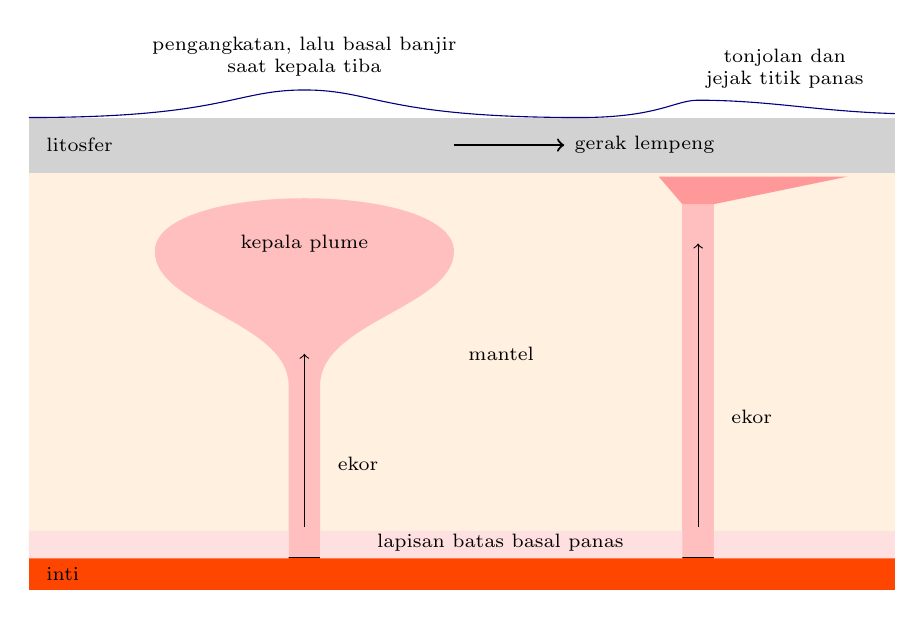
\begin{tikzpicture}[font=\scriptsize, x=1cm, y=1cm]
\fill[orange!12] (0,0) rectangle (11,-5.6);
\fill[gray!35] (0,0) -- (11,0) -- (11,-0.7) -- (0,-0.7) -- cycle;
\fill[red!25] (3.3,-5.6) -- (3.3,-3.4) .. controls (3.3,-2.6) and (1.6,-2.4) .. (1.6,-1.7)
  .. controls (1.6,-0.8) and (5.4,-0.8) .. (5.4,-1.7) .. controls (5.4,-2.4) and (3.7,-2.6) .. (3.7,-3.4) -- (3.7,-5.6) -- cycle;
\fill[red!25] (8.3,-5.6) -- (8.3,-0.75) -- (8.7,-0.75) -- (8.7,-5.6) -- cycle;
\fill[red!40] (8.0,-0.75) -- (8.3,-1.1) -- (8.7,-1.1) -- (10.4,-0.75) -- cycle;
\draw[thick] (0,-5.6) -- (11,-5.6);
\fill[red!45!orange] (0,-5.6) rectangle (11,-6.0);
\fill[red!12] (0,-5.6) rectangle (3.3,-5.25) (3.7,-5.6) rectangle (8.3,-5.25) (8.7,-5.6) rectangle (11,-5.25);
\node[anchor=west] at (0.1,-5.8) {inti};
\node at (3.5,-1.6) {kepala plume};
\node[anchor=west] at (3.8,-4.4) {ekor};
\node[anchor=west] at (8.8,-3.8) {ekor};
\node[anchor=west] at (0.1,-0.35) {litosfer};
\node at (6.0,-3.0) {mantel};
\draw[->] (3.5,-5.2) -- (3.5,-3.0);
\draw[->] (8.5,-5.2) -- (8.5,-1.6);
\draw[->, thick] (5.4,-0.35) -- (6.8,-0.35) node[right] {gerak lempeng};
\draw[blue!50!black] (0,0) .. controls (2.5,0) and (2.6,0.35) .. (3.5,0.35) .. controls (4.4,0.35) and (4.5,0) .. (7,0) .. controls (8,0) and (8.2,0.22) .. (8.5,0.22) .. controls (9.4,0.22) and (10,0.08) .. (11,0.05);
\node[above, align=center] at (3.5,0.4) {pengangkatan, lalu basal banjir\\saat kepala tiba};
\node[above, align=center] at (9.6,0.25) {tonjolan dan\\jejak titik panas};
\node[anchor=west] at (4.3,-5.4) {lapisan batas basal panas};
\end{tikzpicture}

\par\smallskip{\small Plume muda (kiri) naik sebagai kepala besar yang diisi oleh
ekor tipis; ketika kepala menyebar di bawah litosfer, permukaan naik dan basal
banjir dapat meletus. Plume tua (kanan) adalah ekor di bawah lempeng yang bergerak,
memasok tonjolan dan jejak titik panas. Tidak
sesuai skala.}\label{fig:b3:mantle-convection:plume}
\end{omfigure}

Kepala plume adalah bola mantel berdaya apung yang naik melalui mantel kental:
hukum Stokes dari buku fisika, $v = 2\Delta\rho\,ga^2/(9\eta)$, memberi kecepatannya dalam orde
besaran, sebagian kecil meter per tahun untuk kepala dengan lebar beberapa ratus
kilometer (latihan 8), sehingga ia melintasi mantel dalam jutaan tahun.

\section{Penyesuaian isostatik glasial dan viskositas mantel}\label{sec:b3:mantle-convection:gia}

\begin{definition}[Penyesuaian isostatik glasial, viskositas mantel]\label{def:b3:mantle-convection:gia}
Yang disebut \emph{penyesuaian isostatik glasial}\index{penyesuaian isostatik glasial} (GIA)
adalah deformasi lambat Bumi padat, dan perubahan
medan gravitasinya serta permukaan laut, ketika ia kembali menuju kesetimbangan isostatik setelah
lembaran es tumbuh atau mencair. \emph{Viskositas mantel}\index{viskositas mantel}
adalah viskositas efektif $\eta$ yang menghubungkan rayapan mantel yang lambat dan tunak
dengan tegangan yang menggerakkannya, dalam rentang waktu ribuan tahun atau lebih.
\end{definition}

Ketika lembaran es mencair, cekungan yang ditinggalkannya berada di luar
kesetimbangan isostatik: di bawahnya, tekanan mantel lebih rendah daripada di sekitarnya, dan
mantel mengalir masuk untuk mengangkat kembali dasarnya. Hari ini pesisir Teluk Bothnia
naik hingga \qty{10.3}{mm/yr}, di dekat Umeå; Teluk Hudson sekitar
\qty{10}{mm/yr}, tempat es paling tebal, sedangkan daratan di selatan Great
Lakes turun sebesar 1 hingga \qty{2}{mm/yr}, ketika tonjolan yang didorong naik oleh es
di sekitarnya menyusut. Di pesisir, garis pantai lama kini berada di atas laut, yaitu
pantai terangkat dalam kotak lapangan di bawah.
% ledger: vestol19:umea, sella07:gia

\begin{theorem}[Relaksasi setengah-ruang kental]\label{thm:b3:mantle-convection:relaxation}
Cekungan $w(x, t) = w_m(t)\cos(2\pi x/\lambda)$ pada permukaan suatu setengah-ruang
dengan viskositas seragam $\eta$ dan massa jenis $\rho$, yang dibiarkan tanpa beban,
meluruh sebagai $w_m(t) = w_m(0)e^{-t/\tau}$ dengan
\[
  \tau = \frac{4\pi\eta}{\rho g\lambda} .
\]
\end{theorem}

\begin{proof}
Ambil $z$ ke arah bawah, $k = 2\pi/\lambda$, dan cari aliran Stokes yang meluruh
terhadap kedalaman, dengan kecepatan vertikal (ke bawah) $v = (C + Dkz)e^{-kz}\cos kx$.
Kondisi tak-mampumampat memberikan kecepatan horizontal $u = -(D - C - Dkz)e^{-kz}\sin
kx$. Fungsi-fungsi ini memenuhi $\nabla^4 = 0$, seperti halnya setiap aliran Stokes dalam
dua dimensi. Permukaan bebas tidak memikul tegangan geser: $\partial u/\partial
z + \partial v/\partial x = 2k(D - C)\sin kx = 0$ pada $z = 0$, sehingga $D = C$, dan
\[
  v = C(1 + kz)e^{-kz}\cos kx,\quad u = Ckze^{-kz}\sin kx,\quad
  p = 2\eta Cke^{-kz}\cos kx,
\]
tekanan diperoleh dari $\partial p/\partial x = \eta\nabla^2u = -2\eta
Ck^2e^{-kz}\sin kx$ (dan $\partial p/\partial z = \eta\nabla^2v$ terverifikasi). Pada
permukaan $\partial v/\partial z = 0$, sehingga tegangan normal di sana adalah $-p$. Di bawah
cekungan $w$, berat batuan yang hilang menurunkan tekanan sebesar $\rho
gw$: $p(0) = -\rho gw$, sehingga $2\eta Ck = -\rho gw_m$. Permukaan bergerak bersama
fluida: $\mathrm dw_m/\mathrm dt = v(0) = C = -\rho gw_m/(2\eta k)$, yang
solusinya meluruh dengan $\tau = 2\eta k/(\rho g) = 4\pi\eta/(\rho g\lambda)$.
\end{proof}

\begin{definition}[Waktu relaksasi isostatik]\label{def:b3:mantle-convection:relaxation-time}
Yang disebut \emph{waktu relaksasi isostatik}\index{waktu relaksasi isostatik} $\tau$ dari
suatu beban dengan skala horizontal $\lambda$ adalah waktu ketika simpangannya dari
kesetimbangan isostatik meluruh dengan faktor $e$.
\end{definition}

Setengah-ruang seragam merelaksasi cekungan lebar lebih cepat daripada cekungan sempit, dan
aliran di bawah beban dengan panjang gelombang $\lambda$ meluruh terhadap kedalaman sebagai $e^{-kz}$, hingga
kedalaman $\lambda/2\pi$: lembaran es besar mengaduk mantel jauh ke dalam, danau kecil
hanya bagian atasnya. Untuk cekungan selebar \qty{3000}{km} dan $\eta =
\qty{e21}{Pa.s}$, dengan $\rho = \qty{3300}{kg.m^{-3}}$, $\tau = \qty{4.1}{ka}$
(gambar di bawah): setelah sepuluh ribu tahun, $e^{-2.4} = \qty{9}{\percent}$ dari
cekungan yang tersisa, dan karena $\dot w = -w/\tau$, pengangkatan sebesar
\qty{10}{mm/yr} berarti masih ada sekitar \qty{40}{m} kenaikan yang akan datang.

\begin{omfigure}
\begin{tikzpicture}
\begin{groupplot}[group style={group size=1 by 2, vertical sep=2.5cm},
  omrecord, width=0.86\linewidth, height=0.38\linewidth]
\nextgroupplot[xmin=0, xmax=20, ymin=0, ymax=1.05, xlabel={waktu sejak es mencair (ka)},
  ylabel={$w_m(t)/w_m(0)$}, title={(a) peluruhan cekungan selebar \qty{3000}{km}},
  title style={font=\small}, legend style={font=\scriptsize, at={(0.98,0.97)}, anchor=north east}]
% computed in figdata/bachelor-3/gia_relaxation.py; ledger: mitrovica96:haskell, milne04:bifrost
\addplot[red!70!black, thick, densely dashed] table[x=t, y=f20] {figdata/out/bachelor-3-gia_relaxation-decay.dat};
\addlegendentry{$\eta = \qty{e20}{Pa.s}$}
\addplot[omDef, thick] table[x=t, y=f21] {figdata/out/bachelor-3-gia_relaxation-decay.dat};
\addlegendentry{$\eta = \qty{e21}{Pa.s}$}
\addplot[black, thick, densely dotted] table[x=t, y=f22] {figdata/out/bachelor-3-gia_relaxation-decay.dat};
\addlegendentry{$\eta = \qty{e22}{Pa.s}$}
\nextgroupplot[xmode=log, ymode=log, xmin=100, xmax=1e4, ymin=0.01, ymax=1000,
  xlabel={panjang gelombang $\lambda$ (km)}, ylabel={$\tau$ (ka)},
  title={(b) waktu relaksasi terhadap panjang gelombang}, title style={font=\small}]
\addplot[red!70!black, thick, densely dashed] table[x=lam, y=t20] {figdata/out/bachelor-3-gia_relaxation-tau.dat};
\addplot[omDef, thick] table[x=lam, y=t21] {figdata/out/bachelor-3-gia_relaxation-tau.dat};
\addplot[black, thick, densely dotted] table[x=lam, y=t22] {figdata/out/bachelor-3-gia_relaxation-tau.dat};
\end{groupplot}
\end{tikzpicture}

\par\smallskip{\small Relaksasi setengah-ruang kental seragam ($\rho =
\qty{3300}{kg.m^{-3}}$, $g = \qty{9.8}{m.s^{-2}}$) untuk tiga viskositas. (a) Fraksi
cekungan yang tersisa seiring waktu. (b) Waktu relaksasi
$4\pi\eta/(\rho g\lambda)$, lebih panjang untuk beban sempit.}\label{fig:b3:mantle-convection:gia}
\end{omfigure}

Mantel sungguhan tidak seragam, dan pantulannya dibaca dengan model yang melapisinya
dan menambahkan litosfer elastik, yang menahan beban sempit melalui lenturan. Taksiran
pertama, dari pantulan Fennoscandia, memberikan \qty{e21}{Pa.s}, dan
peluruhan pengangkatan di Sungai Angerman di Swedia dan di Teluk Richmond di
Teluk Hudson memberikan rata-rata 0.65 hingga \qty{1.1e21}{Pa.s} dari dasar
litosfer hingga sekitar \qty{1400}{km}, dengan mantel atas sekitar sepuluh kali
lebih rendah viskositasnya daripada mantel bawah. Inversi laju pengangkatan GNSS
Fennoscandia memberikan \omterm{def:b3:mantle-convection:gia}{viskositas mantel} atas sebesar \num{5e20} hingga \qty{e21}{Pa.s}
dalam satu studi dan \num{3.4e20} hingga \qty{5.0e20}{Pa.s} dalam studi lain, serta \omterm{def:b3:mantle-convection:gia}{viskositas
mantel} bawah sebesar \num{5e21} hingga \qty{5e22}{Pa.s}, dan litosfer setebal 93 hingga
\qty{110}{km}. Taksiran-taksiran berbeda dengan faktor dua atau tiga, tetapi keduanya
sepakat pada orde magnitudo dan pada peningkatan seiring kedalaman.
% ledger: mitrovica96:haskell, milne04:bifrost, zhao12:fenno

\begin{definition}[Waktu Maxwell]\label{def:b3:mantle-convection:maxwell}
Yang disebut \emph{waktu Maxwell}\index{waktu Maxwell} suatu bahan dengan viskositas $\eta$
dan modulus geser $\mu$ adalah $\tau_M = \eta/\mu$: beban yang diterapkan dalam waktu jauh lebih singkat daripada
$\tau_M$ menemui padatan elastik; beban yang diterapkan jauh lebih lama menemui fluida kental.
\end{definition}

Dengan $\mu = \rho v_S^2 = \qty{7.7e10}{Pa}$ pada \qty{300}{km} dalam PREM dan $\eta =
\qty{e21}{Pa.s}$, $\tau_M = \qty{1.3e10}{s}$, sekitar empat ratus tahun. Gelombang
seismik, yang berlangsung beberapa detik, melintasi mantel elastik; zaman es, dan
konveksi, mendeformasi fluida. Batuan yang sama adalah keduanya, bergantung pada seberapa lama ia
didorong.
% ledger: data:prem

\begin{inthefield}[Gisik terangkat]
\begin{minipage}[t]{0.55\linewidth}\vspace{0pt}
Di pesisir daratan yang dahulu tertutup es, seorang geomorfolog menemukan
pekerjaan lama laut yang terdampar di pedalaman: punggungan kerikil membulat, takik, dan
platform datar yang dipahat ombak, kini berada di atas jangkauan pasang surut
tertinggi masa kini, kadang berupa tangga beberapa tingkat. Setiap tingkat adalah garis pantai
ketika laut berada di sana; daratan sejak itu terangkat. Cangkang dan kayu hanyut di
gisik lama diberi penanggalan dengan radiokarbon, dan ketinggian aras yang diberi penanggalan,
diratakan ke titik acuan, memberikan pengangkatan terhadap waktu. Ditelusuri sepanjang pesisir,
garis pantai lama ternyata miring, paling tinggi di tempat es paling tebal: kemiringannya
memetakan bentuk pantulan itu.
\end{minipage}\hfill
\begin{minipage}[t]{0.42\linewidth}\vspace{0pt}
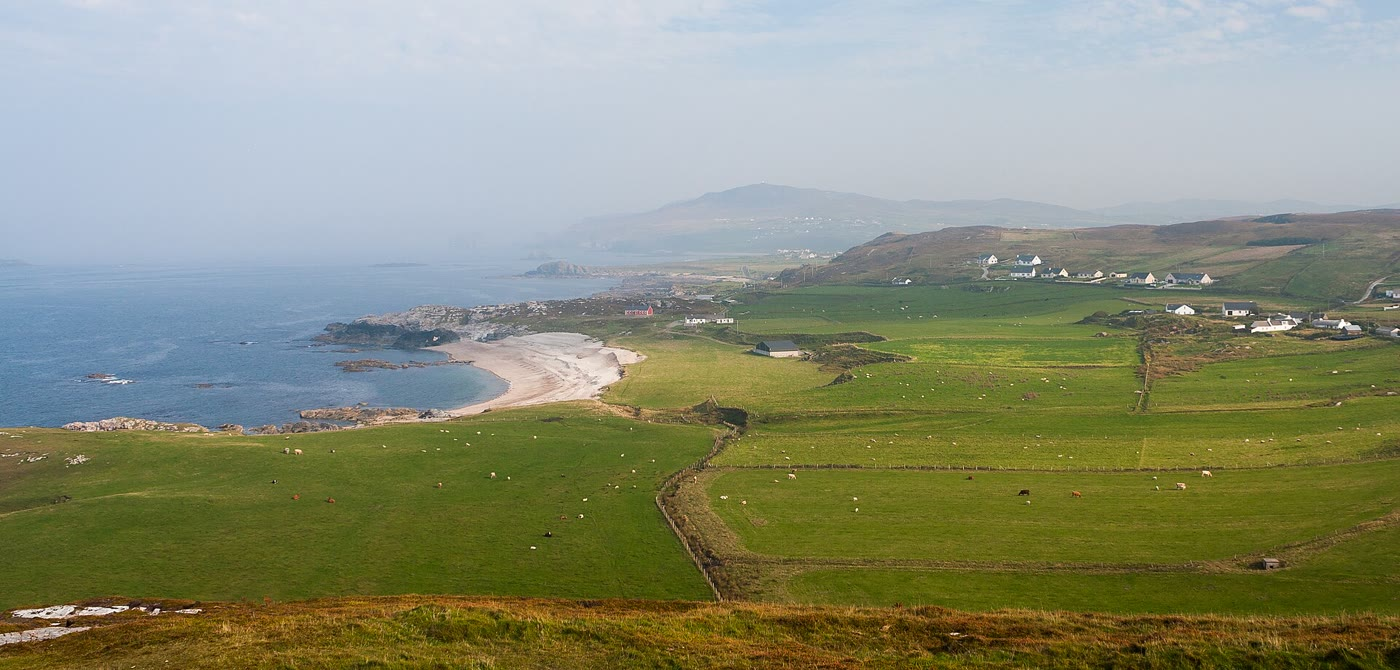
\includegraphics[width=\linewidth]{images/book5/b3-raised-beach-malin.jpg}

{\scriptsize Gisik terangkat di Ballyhillin, Malin Head, di utara
Irlandia: punggungan kerikil garis pantai lama terangkat di atas laut seiring naiknya daratan
setelah lembaran esnya mencair. Foto A.~F.~Borchert, CC BY-SA 4.0.}
\end{minipage}
\end{inthefield}
% ledger: photo:b3-raised-beach

\section{Konveksi seluruh mantel dan struktur dalamnya}

Apakah mantel berkonveksi sebagai satu lapisan, atau dua, di atas dan di bawah
\qty{670}{km} diskontinuitas? Tomografi (\cref{ch:b3:seismology-imaging})
menjawab sebagian: sebagian lempengan mendatar di atas diskontinuitas, sebagian lainnya
menembusnya ke mantel bawah, sehingga massa melintasinya dan kedua lapisan tidak
tertutup satu sama lain. Peningkatan viskositas terhadap kedalaman membuat mantel bawah
mengalir lebih lamban, dan lempengan melambat serta menebal saat memasukinya.

Di dasar mantel, tomografi memperlihatkan dua wilayah luas berkecepatan gelombang S rendah,
di bawah Afrika dan di bawah Pasifik, yakni provinsi kecepatan geser rendah
berskala besar (LLSVPs). Keduanya kemungkinan besar berbeda secara kimiawi dari mantel
di atasnya dan lebih padat, berupa timbunan, bukan plume panas. Provinsi beku besar dan
kimberlit dari beberapa ratus juta tahun terakhir meletus terutama di atas
tepinya, seakan-akan plume naik dari tepi timbunan, tempat lapisan batas panas
di dasar mantel tersapu menuju timbunan itu.
% ledger: st12:llsvp

\section{Latihan}

\begin{exercise}[$\star$]\label{exo:b3:mantle-convection:1}
Hitung \omterm{def:b3:mantle-convection:rayleigh}{bilangan Rayleigh} dari lapisan mantel atas setebal \qty{670}{km} dengan
$\rho = \qty{3500}{kg.m^{-3}}$, $g = \qty{9.9}{m.s^{-2}}$, $\alpha =
\qty{3e-5}{K^{-1}}$, $\Delta T = \qty{1000}{K}$, $\kappa =
\qty{e-6}{m^2.s^{-1}}$ dan $\eta = \qty{5e20}{Pa.s}$. Berapa kali lipat nilai kritisnya
untuk batas bebas-geser?
\end{exercise}

\begin{exercise}[$\star$]\label{exo:b3:mantle-convection:2}
Hitung \omterm{def:b3:mantle-convection:maxwell}{waktu Maxwell} mantel dengan viskositas \qty{e21}{Pa.s} dan modulus geser
\qty{7.7e10}{Pa}, dalam tahun. Apakah mantel merespons secara elastis atau
secara viskos terhadap pasang surut Bumi dua kali sehari, terhadap mencairnya lembaran es, dan terhadap
tenggelamnya lempengan?
\end{exercise}

\begin{exercise}[$\star$]\label{exo:b3:mantle-convection:3}
Dengan $\eta = \qty{e21}{Pa.s}$, $\rho = \qty{3300}{kg.m^{-3}}$ dan $g =
\qty{9.8}{m.s^{-2}}$, hitung waktu relaksasi setengah-ruang seragam untuk
beban dengan panjang gelombang 1000 dan \qty{3000}{km}. Mana yang pulih lebih cepat?
\end{exercise}

\begin{exercise}[$\star$]\label{exo:b3:mantle-convection:4}
Dengan $g = \qty{9.8}{m.s^{-2}}$, $\rho_m = \qty{3300}{kg.m^{-3}}$, $\rho_w =
\qty{1030}{kg.m^{-3}}$, $\alpha = \qty{3.1e-5}{K^{-1}}$, $T_m - T_0 =
\qty{1450}{K}$, $\kappa = \qty{0.8e-6}{m^2.s^{-1}}$ dan \qty{1}{Ma} $=
\qty{3.156e13}{s}$, hitung \omterm{prop:b3:mantle-convection:ridge-push}{gaya dorongan punggung} pada \qty{50}{Ma}. Berapa kali
lebih kecil dibanding tarikan lempengan sebesar \qty{4.6e13}{N.m^{-1}}?
\end{exercise}

\begin{exercise}[$\star\star$]\label{exo:b3:mantle-convection:5}
Sebuah gumpalan mantel selebar \qty{10}{km}, \qty{300}{K} lebih panas daripada
sekelilingnya, naik dengan laju $\rho g\alpha\Delta Td^2/\eta$ (ambil $\rho =
\qty{3300}{kg.m^{-3}}$, $g = \qty{9.8}{m.s^{-2}}$, $\alpha = \qty{3e-5}{K^{-1}}$,
$\eta = \qty{e21}{Pa.s}$, $\kappa = \qty{e-6}{m^2.s^{-1}}$). (a) Hitung
waktu naik melintasi ukurannya sendiri dan waktu difusinya $d^2/\kappa$, lalu tunjukkan
bahwa rasionya sama dengan \omterm{def:b3:mantle-convection:rayleigh}{bilangan Rayleigh-nya}. (b) Apakah ia naik atau mendingin lebih dulu? (c)
Seberapa besar ukurannya agar \omterm{def:b3:mantle-convection:rayleigh}{bilangan Rayleigh-nya} mencapai 657.5?
\end{exercise}

\begin{exercise}[$\star\star$]\label{exo:b3:mantle-convection:6}
Untuk lapisan berkedalaman \qty{2891}{km} pada $\mathrm{Ra} = \num{e7}$, dengan $\kappa =
\qty{e-6}{m^2.s^{-1}}$, $k = \qty{3.1}{W.m^{-1}.K^{-1}}$, $\Delta T =
\qty{1450}{K}$ dan $\mathrm{Ra}_c = 657.5$, hitung ketebalan
lapisan batas, \omterm{def:b3:mantle-convection:nusselt}{bilangan Nusselt}, skala kecepatan dalam \unit{cm/yr}, dan
aliran panas.
\end{exercise}

\begin{exercise}[$\star\star$]\label{exo:b3:mantle-convection:7}
Sebuah tonjolan titik panas rekaan memiliki luas penampang \qty{8e8}{m^2} melintang
jejak, dan lempeng di atasnya bergerak dengan \qty{9}{cm/yr}. Dengan $\rho_m - \rho_w =
\qty{2270}{kg.m^{-3}}$, hitung fluks daya apungnya, dan fluks panasnya dengan $c_p =
\qty{1170}{J.kg^{-1}.K^{-1}}$ dan $\alpha = \qty{3.1e-5}{K^{-1}}$. Berapa pecahan
dari aliran panas Bumi sebesar \qty{46.7}{TW} yang dihasilkannya?
\end{exercise}

\begin{exercise}[$\star\star$]\label{exo:b3:mantle-convection:8}
Sebuah kepala plume berjari-jari \qty{400}{km}, lebih ringan daripada mantel sebesar
\qty{30}{kg.m^{-3}}, naik melalui mantel dengan viskositas \qty{e21}{Pa.s}. Dengan
hukum Stokes, hitung lajunya dalam \unit{m/yr} dan waktu yang dibutuhkan untuk naik sejauh
\qty{2000}{km}.
\end{exercise}

\begin{exercise}[$\star\star$]\label{exo:b3:mantle-convection:9}
Sebuah wilayah tertekan sedalam \qty{300}{m} ketika lembaran esnya mencair, \qty{10}{ka} lalu,
dan berelaksasi dengan $\tau = \qty{4.4}{ka}$. Hitung penurunan yang tersisa hari ini dan
laju pengangkatan saat ini. Bandingkan dengan \qty{10.3}{mm/yr} yang diukur dekat
Umeå.
\end{exercise}

\begin{exercise}[$\star\star\star$]\label{exo:b3:mantle-convection:10}
(a) Dari ekspresi $F_{rp}$ dalam pembuktian
\cref{prop:b3:mantle-convection:ridge-push}, tunjukkan bahwa suku pertama,
$\tfrac12(\rho_m - \rho_w)gw^2$, adalah suku kedua dalam kurung. (b) Tunjukkan bahwa
$\int_0^\infty x\operatorname{erfc}x\,\mathrm dx = 1/4$, dengan integrasi parsial.
(c) Dengan nilai-nilai dari latihan 4, hitung kedua suku pada \qty{100}{Ma}.
\end{exercise}

\begin{exercise}[$\star\star\star$]\label{exo:b3:mantle-convection:11}
Tunjukkan bahwa $f(k) = (\pi^2 + k^2)^3/k^2$ paling kecil pada $k = \pi/\sqrt2$, dengan
nilainya $27\pi^4/4$. Turunkan lebar sepasang sel konveksi pada awal
konveksi, dalam satuan $d$, dan lebar satu sel.
\end{exercise}

\begin{exercise}[$\star\star\star$]\label{exo:b3:mantle-convection:12}
Sebuah lempeng sepanjang \qty{6000}{km} bergerak dengan \qty{6}{cm/yr} di atas lapisan mantel
setebal \qty{150}{km}, dengan viskositas \qty{e20}{Pa.s}, yang dasarnya diam. (a)
Hitung \omterm{def:b3:mantle-convection:basal-drag}{seretan basal} dalam \unit{MPa} dan gaya seret per satuan panjang lempeng.
(b) Bandingkan dengan dorongan punggung sebesar \qty{3.8e12}{N.m^{-1}} dan tarikan lempengan sebesar
\qty{4.6e13}{N.m^{-1}}. (c) Jika sepersepuluh tarikan lempengan mencapai lempeng,
pada laju berapa seretan menyeimbangkan gaya penggeraknya?
\end{exercise}

\section{Soal: Pantulan Danau Ardo}

\begin{problem}[{Soal akhir pekan --- pantulan cekungan danau rekaan,
viskositas mantel di bawahnya, dan konveksi yang dimungkinkan
oleh viskositas itu}]
\label{pb:b3:mantle-convection:1}
% values: calc/ch06.py; gia_relaxation.py, convection_scaling.py
Danau Ardo, danau rekaan, mengisi cekungan selebar \qty{250}{km}, dibendung oleh
lembaran es, dengan kedalaman \qty{300}{m} selama sekitar lima puluh ribu tahun. Empat belas
ribu tahun lalu bendungan es jebol dan danau surut dalam beberapa minggu.
Garis pantai tertinggi, yang dulu datar saat terbentuk, kini miring; garis pantai
bertanggal dari danau-danau kecil yang tersisa di cekungan memberikan pengangkatan pusat
sejak pengeringan, relatif terhadap tepi yang hampir tidak bergerak:

\smallskip
\begin{center}\small
\begin{tabular}{lcccccc}
\hline
waktu sejak pengeringan (ka) & 1 & 2 & 4 & 6 & 9 & 14\\
pengangkatan pusat (m) & 11.5 & 21.6 & 38.0 & 50.5 & 64.0 & 77.2\\
\hline
\end{tabular}
\end{center}
\smallskip

Ambil $\rho_w = \qty{1000}{kg.m^{-3}}$, $\rho_m = \qty{3300}{kg.m^{-3}}$, $g =
\qty{9.8}{m.s^{-2}}$, \qty{1}{yr} $= \qty{3.156e7}{s}$, dan perlakukan mantel sebagai
ruang setengah kental seragam.

\medskip\noindent\textbf{Bagian I --- Beban.}
\begin{enumerate}
  \item Hitung tekanan danau pada dasarnya.
  \item Hitung penekanan dasar pada kesetimbangan isostatik, dan jelaskan
        mengapa massa jenis mantel, bukan kerak, muncul di dalamnya.
  \item Anggap danau sebagai cakram, lalu hitung massa airnya.
  \item Jelaskan mengapa garis pantai tertinggi kini miring, dan hitung kemiringan
        rata-ratanya dari tepi ke pusat, dalam meter per kilometer.
  \item Penekanan diperlakukan sebagai satu harmonik yang setengah tertekannya, dari
        $-\lambda/4$ sampai $\lambda/4$, membentang di seluruh danau. Berikan $\lambda$ dan $k =
        2\pi/\lambda$.
  \item Pada kedalaman berapa aliran di bawah beban seperti itu meluruh dengan faktor
        $e$?
\end{enumerate}

\medskip\noindent\textbf{Bagian II --- Waktu relaksasi.}
\begin{enumerate}[resume]
  \item Dengan anggapan danau telah mencapai kesetimbangan, hitung penekanan yang tersisa
        pada setiap tanggal dalam tabel.
  \item Tunjukkan bahwa, jika penekanan meluruh secara eksponensial, logaritmanya turun
        secara linear terhadap waktu.
  \item Hitung $\tau$ dari tanggal 1 dan \qty{14}{ka}.
  \item Prediksikan pengangkatan pada \qty{6}{ka} dengan $\tau$ tersebut, dan bandingkan dengan
        tabel.
  \item Hitung penekanan yang tersisa hari ini dan laju pengangkatan pusat saat ini,
        dalam \unit{mm/yr}.
  \item Berapa banyak pengangkatan yang masih akan terjadi?
  \item Dalam berapa tahun lagi laju pengangkatan akan turun di bawah
        \qty{0.5}{mm/yr}?
\end{enumerate}

\medskip\noindent\textbf{Bagian III --- Viskositas.}
\begin{enumerate}[resume]
  \item Hitung viskositas ruang setengah dari $\tau$.
  \item Bandingkan dengan \omterm{def:b3:mantle-convection:gia}{viskositas mantel} atas sebesar \num{3.4e20} sampai
        \qty{1e21}{Pa.s} yang ditemukan di bawah Fennoskandia. Bagian mantel mana
        yang tersampel oleh pantulan Danau Ardo?
  \item Dengan viskositas itu, hitung waktu relaksasi beban
        dengan panjang gelombang \qty{3000}{km}. Mengapa lembaran es sungguhan sebesar itu
        akan meluruh lebih lambat daripada ini?
  \item Apa yang dilakukan litosfer elastik, yang diabaikan di sini, terhadap pantulan
        beban yang hanya selebar \qty{250}{km}?
  \item Hitung \omterm{def:b3:mantle-convection:maxwell}{waktu Maxwell} mantel dengan $\mu = \qty{7.7e10}{Pa}$, lalu
        nyatakan apakah model kental itu dapat dibenarkan.
  \item Periksa asumsi pertanyaan 7: berapa bagian dari penekanan kesetimbangan
        yang tercapai selama danau berdiri?
  \item Berapa besar $\log_{10}\eta$ akan berubah jika $\lambda$ diambil sebagai
        \qty{250}{km}?
\end{enumerate}

\medskip\noindent\textbf{Bagian IV --- Konveksi.} Ambil lapisan mantel atas dengan kedalaman
\qty{670}{km}, dengan $\rho = \qty{3700}{kg.m^{-3}}$, $g =
\qty{9.9}{m.s^{-2}}$, $\alpha = \qty{3.1e-5}{K^{-1}}$, $\Delta T =
\qty{1450}{K}$, $\kappa = \qty{e-6}{m^2.s^{-1}}$, $k = \qty{3.1}{W.m^{-1}.K^{-1}}$
dan viskositas Bagian III.
\begin{enumerate}[resume]
  \item Hitung \omterm{def:b3:mantle-convection:rayleigh}{bilangan Rayleigh} lapisan itu.
  \item Berapa kali lipat nilai kritisnya ($\mathrm{Ra}_c = 657.5$)?
  \item Hitung tebal lapisan batas dan \omterm{def:b3:mantle-convection:nusselt}{bilangan Nusselt}.
  \item Hitung skala kecepatan dalam \unit{cm/yr}, dan bandingkan dengan laju
        lempeng sebesar 1 sampai \qty{7.5}{cm/yr}.
  \item Hitung aliran panas, dan berikan dua alasan mengapa nilai itu berada di bawah
        rata-rata Bumi, \qty{92}{mW.m^{-2}}.
  \item Berikan \omterm{def:b3:mantle-convection:gia}{viskositas mantel} atas di bawah Danau Ardo sebagai $\log_{10}$ dari
        $\eta$ dalam \unit{Pa.s}.
\end{enumerate}
\end{problem}
